% Generated by LitigCharts.PublicationFigures. Captions and provenance are sidecars.
\documentclass[10pt,tikz,border=5pt]{standalone}
\usepackage{lmodern}
\usetikzlibrary{patterns,patterns.meta}
\begin{document}
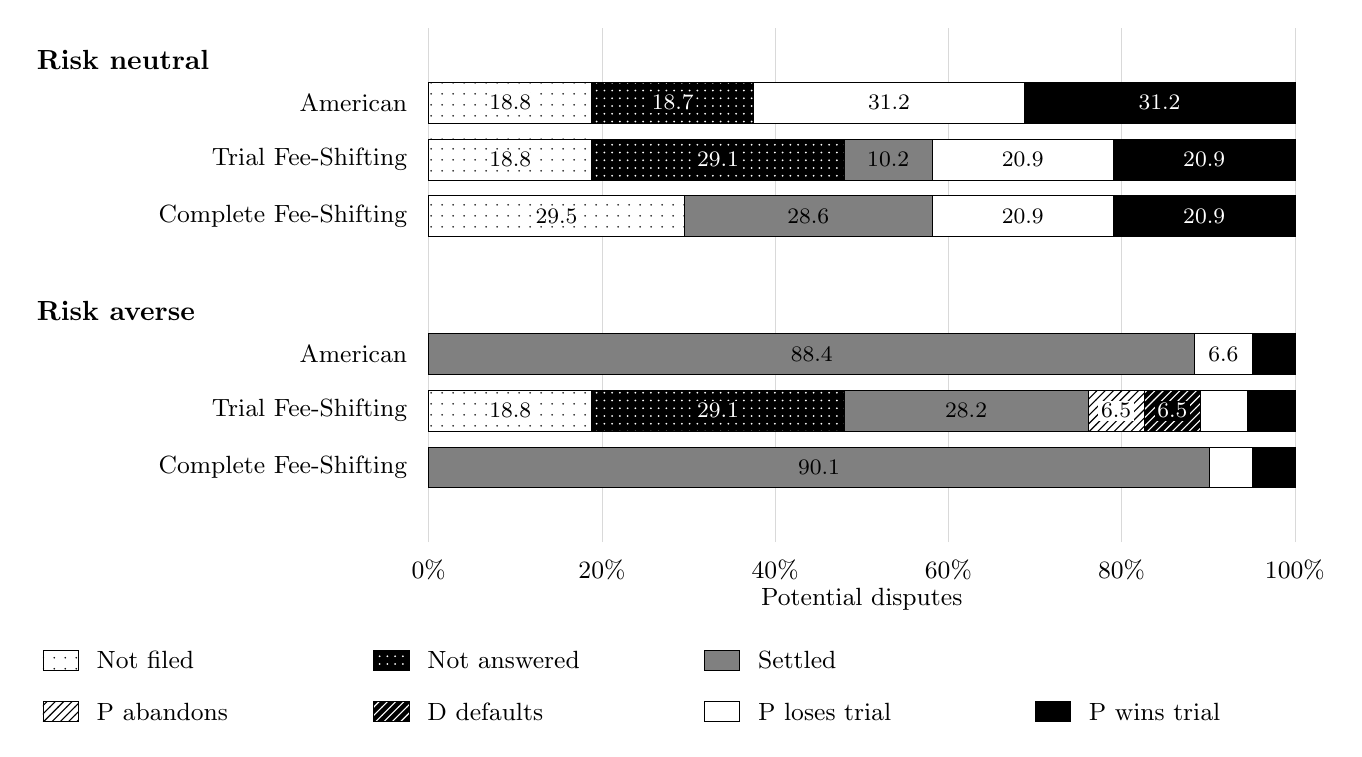
\begin{tikzpicture}[font=\small]\draw[black!15,line width=.2pt] (5.1,.65) -- (5.1,7.18);
\node[anchor=north] at (5.1,.55) {0\%};
\draw[black!15,line width=.2pt] (7.3,.65) -- (7.3,7.18);
\node[anchor=north] at (7.3,.55) {20\%};
\draw[black!15,line width=.2pt] (9.5,.65) -- (9.5,7.18);
\node[anchor=north] at (9.5,.55) {40\%};
\draw[black!15,line width=.2pt] (11.7,.65) -- (11.7,7.18);
\node[anchor=north] at (11.7,.55) {60\%};
\draw[black!15,line width=.2pt] (13.9,.65) -- (13.9,7.18);
\node[anchor=north] at (13.9,.55) {80\%};
\draw[black!15,line width=.2pt] (16.1,.65) -- (16.1,7.18);
\node[anchor=north] at (16.1,.55) {100\%};
\node[anchor=west,font=\bfseries] at (0,6.78) {\mbox{Risk} \mbox{neutral}};
\node[anchor=east] at (4.95,6.23) {American};
\path[preaction={fill=white,draw=none},pattern={Dots[distance=4pt,radius=.35pt]},pattern color=black,draw=black,line width=.25pt] (5.1,5.97) rectangle (7.17119,6.49);
\node[text=black,fill=white,font=\footnotesize,inner sep=1pt] at (6.135595,6.23) {18.8};
\path[preaction={fill=black,draw=none},pattern={Dots[distance=2.8pt,radius=.35pt]},pattern color=white,draw=black,line width=.25pt] (7.17119,5.97) rectangle (9.227585,6.49);
\node[text=white,fill=black,font=\footnotesize,inner sep=1pt] at (8.199388,6.23) {18.7};
\path[fill=white,draw=black,line width=.25pt] (9.227585,5.97) rectangle (12.663842,6.49);
\node[text=black,fill=none,font=\footnotesize,inner sep=1pt] at (10.945714,6.23) {31.2};
\path[fill=black,draw=black,line width=.25pt] (12.663842,5.97) rectangle (16.1,6.49);
\node[text=white,fill=none,font=\footnotesize,inner sep=1pt] at (14.381921,6.23) {31.2};
\node[anchor=east] at (4.95,5.51) {Trial Fee-Shifting};
\path[preaction={fill=white,draw=none},pattern={Dots[distance=4pt,radius=.35pt]},pattern color=black,draw=black,line width=.25pt] (5.1,5.25) rectangle (7.17119,5.77);
\node[text=black,fill=white,font=\footnotesize,inner sep=1pt] at (6.135595,5.51) {18.8};
\path[preaction={fill=black,draw=none},pattern={Dots[distance=2.8pt,radius=.35pt]},pattern color=white,draw=black,line width=.25pt] (7.17119,5.25) rectangle (10.376777,5.77);
\node[text=white,fill=black,font=\footnotesize,inner sep=1pt] at (8.773984,5.51) {29.1};
\path[fill=black!50,draw=black,line width=.25pt] (10.376777,5.25) rectangle (11.493387,5.77);
\node[text=black,fill=none,font=\footnotesize,inner sep=1pt] at (10.935082,5.51) {10.2};
\path[fill=white,draw=black,line width=.25pt] (11.493387,5.25) rectangle (13.796721,5.77);
\node[text=black,fill=none,font=\footnotesize,inner sep=1pt] at (12.645054,5.51) {20.9};
\path[fill=black,draw=black,line width=.25pt] (13.796721,5.25) rectangle (16.100011,5.77);
\node[text=white,fill=none,font=\footnotesize,inner sep=1pt] at (14.948366,5.51) {20.9};
\node[anchor=east] at (4.95,4.79) {Complete Fee-Shifting};
\path[preaction={fill=white,draw=none},pattern={Dots[distance=4pt,radius=.35pt]},pattern color=black,draw=black,line width=.25pt] (5.1,4.53) rectangle (8.34555,5.05);
\node[text=black,fill=white,font=\footnotesize,inner sep=1pt] at (6.722775,4.79) {29.5};
\path[fill=black!50,draw=black,line width=.25pt] (8.34555,4.53) rectangle (11.493376,5.05);
\node[text=black,fill=none,font=\footnotesize,inner sep=1pt] at (9.919463,4.79) {28.6};
\path[fill=white,draw=black,line width=.25pt] (11.493376,4.53) rectangle (13.79671,5.05);
\node[text=black,fill=none,font=\footnotesize,inner sep=1pt] at (12.645043,4.79) {20.9};
\path[fill=black,draw=black,line width=.25pt] (13.79671,4.53) rectangle (16.1,5.05);
\node[text=white,fill=none,font=\footnotesize,inner sep=1pt] at (14.948355,4.79) {20.9};
\node[anchor=west,font=\bfseries] at (0,3.59) {\mbox{Risk} \mbox{averse}};
\node[anchor=east] at (4.95,3.04) {American};
\path[fill=black!50,draw=black,line width=.25pt] (5.1,2.78) rectangle (14.827674,3.3);
\node[text=black,fill=none,font=\footnotesize,inner sep=1pt] at (9.963837,3.04) {88.4};
\path[fill=white,draw=black,line width=.25pt] (14.827674,2.78) rectangle (15.557711,3.3);
\node[text=black,fill=none,font=\footnotesize,inner sep=1pt] at (15.192693,3.04) {6.6};
\path[fill=black,draw=black,line width=.25pt] (15.557711,2.78) rectangle (16.099998,3.3);
\node[anchor=east] at (4.95,2.32) {Trial Fee-Shifting};
\path[preaction={fill=white,draw=none},pattern={Dots[distance=4pt,radius=.35pt]},pattern color=black,draw=black,line width=.25pt] (5.1,2.06) rectangle (7.17119,2.58);
\node[text=black,fill=white,font=\footnotesize,inner sep=1pt] at (6.135595,2.32) {18.8};
\path[preaction={fill=black,draw=none},pattern={Dots[distance=2.8pt,radius=.35pt]},pattern color=white,draw=black,line width=.25pt] (7.17119,2.06) rectangle (10.376777,2.58);
\node[text=white,fill=black,font=\footnotesize,inner sep=1pt] at (8.773984,2.32) {29.1};
\path[fill=black!50,draw=black,line width=.25pt] (10.376777,2.06) rectangle (13.473574,2.58);
\node[text=black,fill=none,font=\footnotesize,inner sep=1pt] at (11.925176,2.32) {28.2};
\path[preaction={fill=white,draw=none},pattern={north east lines},pattern color=black,draw=black,line width=.25pt] (13.473574,2.06) rectangle (14.186976,2.58);
\node[text=black,fill=white,font=\footnotesize,inner sep=1pt] at (13.830275,2.32) {6.5};
\path[preaction={fill=black,draw=none},pattern={north east lines},pattern color=white,draw=black,line width=.25pt] (14.186976,2.06) rectangle (14.90037,2.58);
\node[text=white,fill=black,font=\footnotesize,inner sep=1pt] at (14.543673,2.32) {6.5};
\path[fill=white,draw=black,line width=.25pt] (14.90037,2.06) rectangle (15.500191,2.58);
\path[fill=black,draw=black,line width=.25pt] (15.500191,2.06) rectangle (16.100003,2.58);
\node[anchor=east] at (4.95,1.6) {Complete Fee-Shifting};
\path[fill=black!50,draw=black,line width=.25pt] (5.1,1.34) rectangle (15.015851,1.86);
\node[text=black,fill=none,font=\footnotesize,inner sep=1pt] at (10.057926,1.6) {90.1};
\path[fill=white,draw=black,line width=.25pt] (15.015851,1.34) rectangle (15.557931,1.86);
\path[fill=black,draw=black,line width=.25pt] (15.557931,1.34) rectangle (16.100003,1.86);
\node at (10.6,-.08) {Potential disputes};
\path[preaction={fill=white,draw=none},pattern={Dots[distance=4pt,radius=.35pt]},pattern color=black,draw=black,line width=.25pt] (0.2,-0.98) rectangle (0.65,-0.72);
\node[anchor=west] at (0.76,-0.85) {Not filed};
\path[preaction={fill=black,draw=none},pattern={Dots[distance=2.8pt,radius=.35pt]},pattern color=white,draw=black,line width=.25pt] (4.4,-0.98) rectangle (4.85,-0.72);
\node[anchor=west] at (4.96,-0.85) {Not answered};
\path[fill=black!50,draw=black,line width=.25pt] (8.6,-0.98) rectangle (9.05,-0.72);
\node[anchor=west] at (9.16,-0.85) {Settled};
\path[preaction={fill=white,draw=none},pattern={north east lines},pattern color=black,draw=black,line width=.25pt] (0.2,-1.63) rectangle (0.65,-1.37);
\node[anchor=west] at (0.76,-1.5) {P abandons};
\path[preaction={fill=black,draw=none},pattern={north east lines},pattern color=white,draw=black,line width=.25pt] (4.4,-1.63) rectangle (4.85,-1.37);
\node[anchor=west] at (4.96,-1.5) {D defaults};
\path[fill=white,draw=black,line width=.25pt] (8.6,-1.63) rectangle (9.05,-1.37);
\node[anchor=west] at (9.16,-1.5) {P loses trial};
\path[fill=black,draw=black,line width=.25pt] (12.8,-1.63) rectangle (13.25,-1.37);
\node[anchor=west] at (13.36,-1.5) {P wins trial};
\end{tikzpicture}
\end{document}
